\section{Case Studies}\label{sec:case-studies}

In this section, we introduce three motivating datasets of complex objects -- the Glaucoma dataset, the Proteomic Gels dataset and the MNIST digits dataset (Figure \ref{fig:combined-data-objects} (a)--(c)).
We apply our CLaRe framework to select among three latent feature representation methods -- Principal Components Analysis (PCA), the Discrete Wavelet Transform (DWT) and an autoencoder (AE) -- for each dataset.
We then conclude in Section \ref{sec:sample-size-experiment} by presenting the results of an experiment where we artificially decimate the sample size of the Glaucoma dataset to demonstrate how the optimal latent representation can depend on sample size, with more flexible empirical methods (e.g. PCA) working well when there is enough data to reliably estimate the latent features, and fixed methods (e.g. wavelets) performing better when there is not enough data.
For all applications, we use a tolerance level of $\epsilon = 0.05$, an attainment rate of $\alpha=0.95$ and employ the complement of the squared correlation as our loss function.
Implementation details for PCA, DWT and the AE are detailed in our description of the software implementation (Section \ref{sec:software}).

\begin{figure}
    \centering
    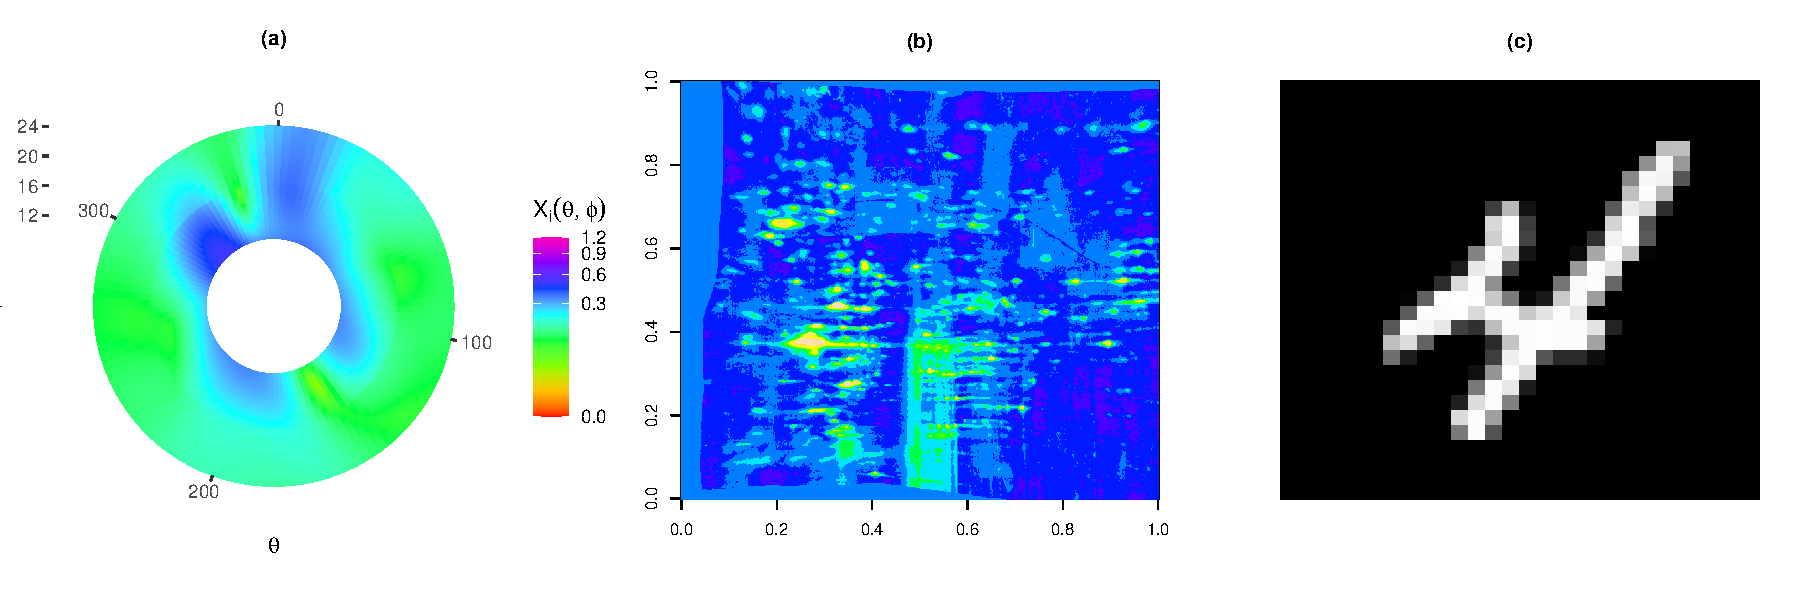
\includegraphics[width=1\textwidth]{figures/data-plot.pdf}
    \caption{
    A sample observation from each of our three motivating datasets.
    \textbf{(a)}: A sample glaucoma image, representing a polar azimuthal projection of MPS functions for a single eye at one IOP level.
    \textbf{(b)}: A sample 2D gel electrophoresis image, showing proteomic content in the brain tissue of a rat.
    \textbf{(c)}: A sample MNIST digit image, which is a $28 \times 28$ pixel greyscale image of a single handwritten digit.}
    \label{fig:combined-data-objects}
\end{figure}



\subsection{Glaucoma Data}

Glaucoma is considered a leading factor in blindness. It is characterized by damage to the optic nerve, which can be induced by \emph{intraocular pressure (IOP)}. 
To investigate proposed hypotheses about the relationship between glaucoma and IOP, \textcite{fazio_age-related_2014} developed instrumentation to measure the mechanical strain on the scleral surface of the eye at different levels of IOP. 
The measurements were summarized for each location at different locations on the scleral surface of the eye as \emph{maximum principal strain} (MPS). MPS was computed on 34 eyes from 19 normal human donors. It was measured in the posterior globe of both eyes on a partial spherical domain with $120$ circumferential locations $\upsilon \in (0^{\circ}, 360^{\circ})$ and $120$ meridional locations $\theta \in (9^{\circ}, 24^{\circ})$.
These measurements were taken at 9 different IOP levels.
One study goal for this dataset was to test the hypothesis that scleral strain decreases with age thereby leaving the optic nerve head susceptible to damage which could be a contributing factor in the development of glaucoma \parencite{lee_bayesian_2019}.
% In this work, we use a simulated copy of the real dataset that was made publicly available by \textcite{lee_bayesian_2019}\footnote{\url{https://www.tandfonline.com/doi/suppl/10.1080/01621459.2018.1476242}}.
Figure \ref{fig:combined-data-objects} (a) displays a two-dimensional polar azimuthal projection of a single observation from the Glaucoma data.

We let $X_i(t)$ denote the MPS function for a single eye at a specific IOP level so that $i = 1, \dots, N = 306$ ($34$ eyes at $9$ IOP levels).
The data lives on a domain $\mathcal{T}$ which is the portion of the sphere defined by $(\upsilon, \theta)$ for $\upsilon \in (0^{\circ}, 360^{\circ})$ and $\theta \in (9^{\circ}, 24^{\circ})$.
Therefore, each observation $X_i(t)$ is recorded a common grid of size $T = 14400$.
The recordings are indexed by the $14400$-dimensional vector $\mathbf{t} = \boldsymbol{\upsilon} \times \boldsymbol{\theta}$, where $\boldsymbol{\upsilon}$ represents $120$ equally-spaced measurements of $\upsilon$ along $(0^{\circ}, 360^{\circ})$ and $\boldsymbol{\theta}$ represents $120$ equally-spaced measurements of $\theta$ along $(9^{\circ}, 24^{\circ})$.
We denote the vector of measurements for the $i$th observation as $X_i(\mathbf{t})$, so that the full dataset can be represented by the $N \times T$ data matrix $\mathbf{X}$, containing $X_1(\mathbf{t}), \dots, X_N(\mathbf{t})$ in its rows.

Figure \ref{fig:eye-results} displays the summary plot from the application of \texttt{GLaRe()} to the Glaucoma data.
PCA is the most suitable latent feature representation method for this dataset because it achieves the qualifying criterion with qualifying dimension $qd=51$, whereas DWT and AE do not achieve the qualifying criterion for $K \leq 301$.
A grid of equally-spaced values from $1$ to $301$ in increments of $10$ was used for the latent feature dimensions.
Although it was possible to use larger latent feature dimensions for the DWT and AE, it was deemed unnecessary because the qualifying criterion was achieved for PCA with a qualifying dimension $qd=51$ and is the favored method for this dataset.
PCA provides dimension reduction of $282:1$ ($T = 14400$ to $qd = 51$).
The computation times for PCA, DWT and AE were $1.6$, $1.7$ and $67.4$ minutes, respectively.


\begin{figure}
    \centering
    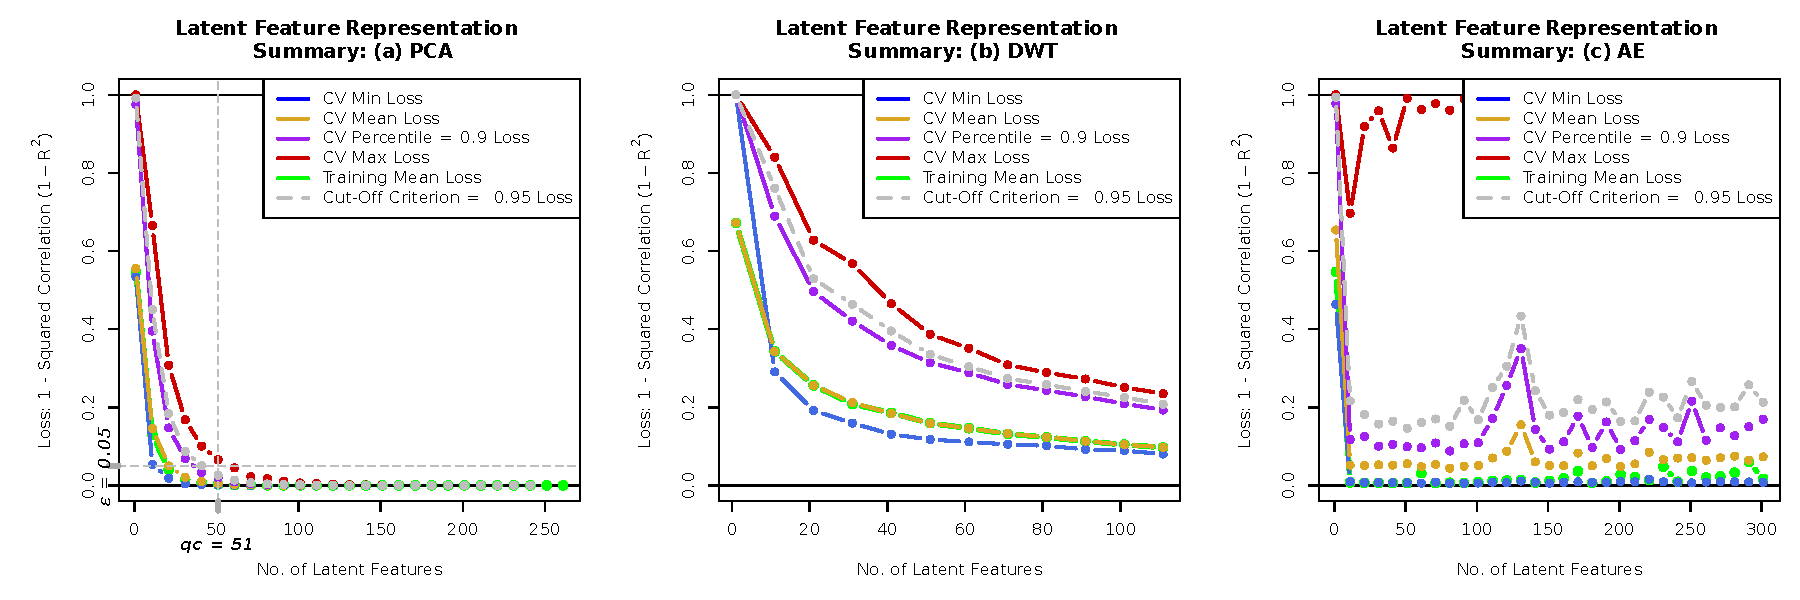
\includegraphics[width=1\textwidth]{figures/eye-results.pdf}
    \caption{Summary \texttt{GLaRe()} plot for the Glaucoma data. A grid of equally-spaced values from $1$ to $301$ in increments of $10$ was used for the latent feature dimensions. 
    % \textbf{Note}: For PCA, the maximum number of non-zero eigenvalues was $\leq361$ so only results for $K \leq 361$ are displayed on the summary plot.
    The legend for plots (b) and (c) has been suppressed so that it does not mask the worst-case observation and because it is identical to the legend for plot (a).}
    \label{fig:eye-results}
\end{figure}

\subsection{Proteomic Gels Data}

In neurobiology, a particularly important issue is the identification of changes responsible for the transition from non-dependent drug use to addiction which is characterized by drug intake behavior. Studies done on rats have shown that rats given a 6-12 hours/day access to cocaine or heroin have significant increase in drug intake while rats given 1 hour/day access kept the same level of intake over time.
The corresponding neurochemical changes in the extended part of the brain amygdala relate to cellular effects that affect protein expression and function which can be detected via proteomic analysis. To study this phenomenon, experiments were done on rats in which the rats were trained to get cocaine by pressing a lever: 6 rats were given 1hour/day access, 7 rats were given 6 hours /day access and 8 rats were used for control with no access to cocaine. The rats were euthanized after some time, and their brains studied \parencite{morris_pinnacle_2008}. 
Two-dimensional gel electrophoresis was used to study the proteomic content in the brain tissues. 
Between two and three gels were obtained from each rat and brain region, resulting in a dataset of 53 gel images from 21 rats.
Each gel image has $556,206$ pixel intensities observed on a $646 \times 861$ grid. 
A research goal for this dataset was to study the proteins which are differentially expressed in the brains of rats that were exposed to cocaine for a long time versus those that were not.
This can be done by finding regions in the gel images where image intensity is significantly different across groups \parencite{morris_statistical_2012}. 
Figure \ref{fig:combined-data-objects} (b) displays a single gel image observation.

We denote a single observation from the Proteomic Gels dataset as $X_i(t)$, where $i=1, \dots, N = 53$.
Here, $t$ represents a location $(t_1, t_2)$ in the two-dimensional Euclidean domain defined by the Cartesian product $\mathcal{T} = [0, 1] \times [0, 1]$.
Measurements of each observation are made at the vector of locations $\mathbf{t} = \mathbf{t}_1 \times \mathbf{t}_2$ where $\mathbf{t}_1$ and $\mathbf{t}_2$ represent vectors of $646$ and $861$ equally-spaced points along $[0, 1]$, respectively.
Then $X_i (\mathbf{t})$ denotes the $T = 556206 ( = 646 \times 861)$-dimensional vector containing the measurements of the $i$th observation at the locations in $\mathbf{t}$, and the $N \times T$ data matrix $\mathbf{X}$ contains $X_1 (\mathbf{t}), \dots, X_N (\mathbf{t})$ in its rows.

Figure \ref{fig:gels-results} displays the summary plot from the application of \texttt{GLaRe()} to the Proteomic Gels data.
Because this dataset only contains $N=53$ observations, the maximum possible latent dimension for PCA is $52$ and PCA does not achieve the qualifying criterion for $K \leq 52$.
Due to computational constraints, we ran the AE for the same range of candidate latent feature dimensions, and it did not achieve the qualifying criterion.
In contrast, the maximum latent dimension for the DWT is not constrained and hence we run \texttt{GLaRe()} on a grid of equally-spaced values from $1$ to $8000$ in increments of $100$.
The qualifying dimension for the DWT is $qd=7801$.
Hence, the DWT is the favored representation method for the Proteomic Gels dataset and it provides a compression ratio of $71:1$ ($T = 556206$ to $qd = 7801$).
The computation times for PCA, DWT and AE were $0.9$, $47.6$ and $109.6$ minutes, respectively.


\begin{figure}
    \centering
    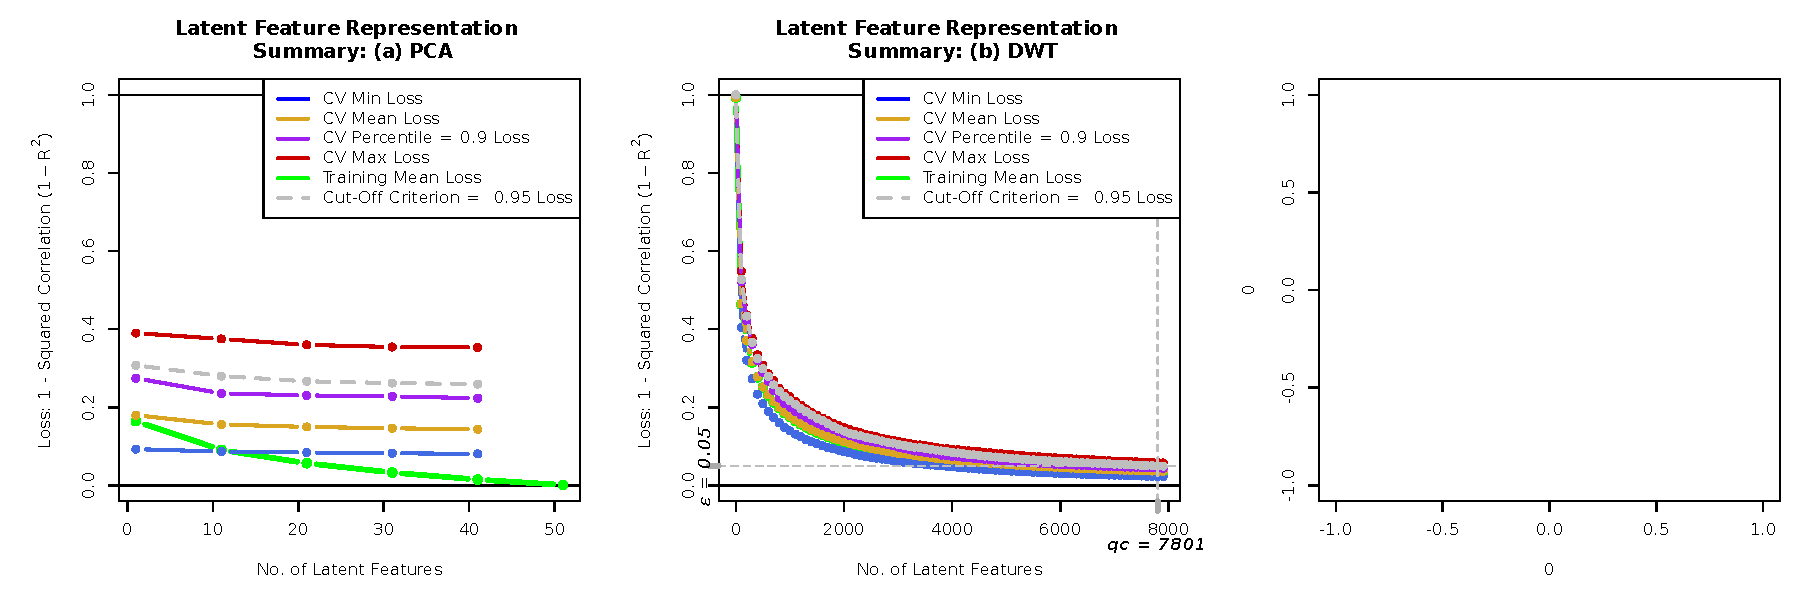
\includegraphics[width=1\linewidth]{figures/gels-results.pdf}
    \caption{Summary \texttt{GLaRe()} plot for the Proteomic Gels data. For PCA and AE, a grid of equally-spaced values from $1$ to $53$ in increments of $10$ was used for the latent feature dimensions.
    For the DWT,  a grid of equally-spaced values from $1$ to $8000$ in increments of $10$ was used for the latent feature dimensions.}
    \label{fig:gels-results}
\end{figure}


\subsection{MNIST Digits Data}

The MNIST (Modified National Institute of Standards and Technology) database of handwritten digits was compiled by \textcite{lecun_mnist_1998}, from a larger collection of images from the National Institute of Standards and Technology (NIST).
It comprises a training set of $60000$ images and a test set of $10000$ images, representing hand-written digits from $0$ to $9$ (i.e., $10$ distinct digits/classes).
The original black and white images from NIST were modified into $28 \times 28$ pixel greyscale images.
The MNIST dataset has been employed extensively in computer vision and deep learning applications as a test case for image reconstruction and digit identification/ classification models.
The dataset can be represented in an $N \times T$ matrix $\mathbf{X}$, where $N = 60000$ (in the case of the training set) and $T= 784$ $(= 28 \times 28)$.
We let $X_i(t)$ represent the value of the $i$th greyscale image at pixel location $t$, where $t \in \mathbf{t} = \{1, \dots, 28\} \times \{1, \dots, 28\}$.
Then the $i$th row of the data matrix $\mathbf{X}$ contains the $784$-dimensional vector $X_i(\mathbf{t})$, i.e., measurements of the $i$th observation at the vector of pixel locations in $\mathbf{t}$.
We normalise the greyscale images so that $X_i(t) \in [0, 1]$ for all $t \in \mathbf{t}$ and $i = 1, \dots, N$. 
Figure \ref{fig:combined-data-objects} (c) displays a single digit from the MNIST dataset.
The full dataset (training and test) is publicly available in the \pkg{keras} \proglang{R} package \parencite{kalinowski_keras_2024} and can be loaded using the \texttt{dataset\_mnist()} function.

Figure \ref{fig:mnist-results} displays the summary plot from the application of \texttt{GLaRe()} to the MNIST data.
A grid of equally-spaced values from $1$ to $381$ in increments of $20$ was used for the latent feature dimensions.
All three latent feature representation methods achieve the qualifying criterion within this range: $qd = 201$ for PCA, $qd = 321$ for the DWT and $qd = 101$ for the AE.
Hence, the AE is the preferred method for this dataset because it provides the most compact (i.e., smallest qd) representation.
The AE has a compression ratio of $8:1$ ($T = 784$ to $K = 101$).
The computation times for PCA, DWT and AE were $16.2$, $27.4$ and $1115.3$ minutes, respectively.

\begin{figure}
    \centering
    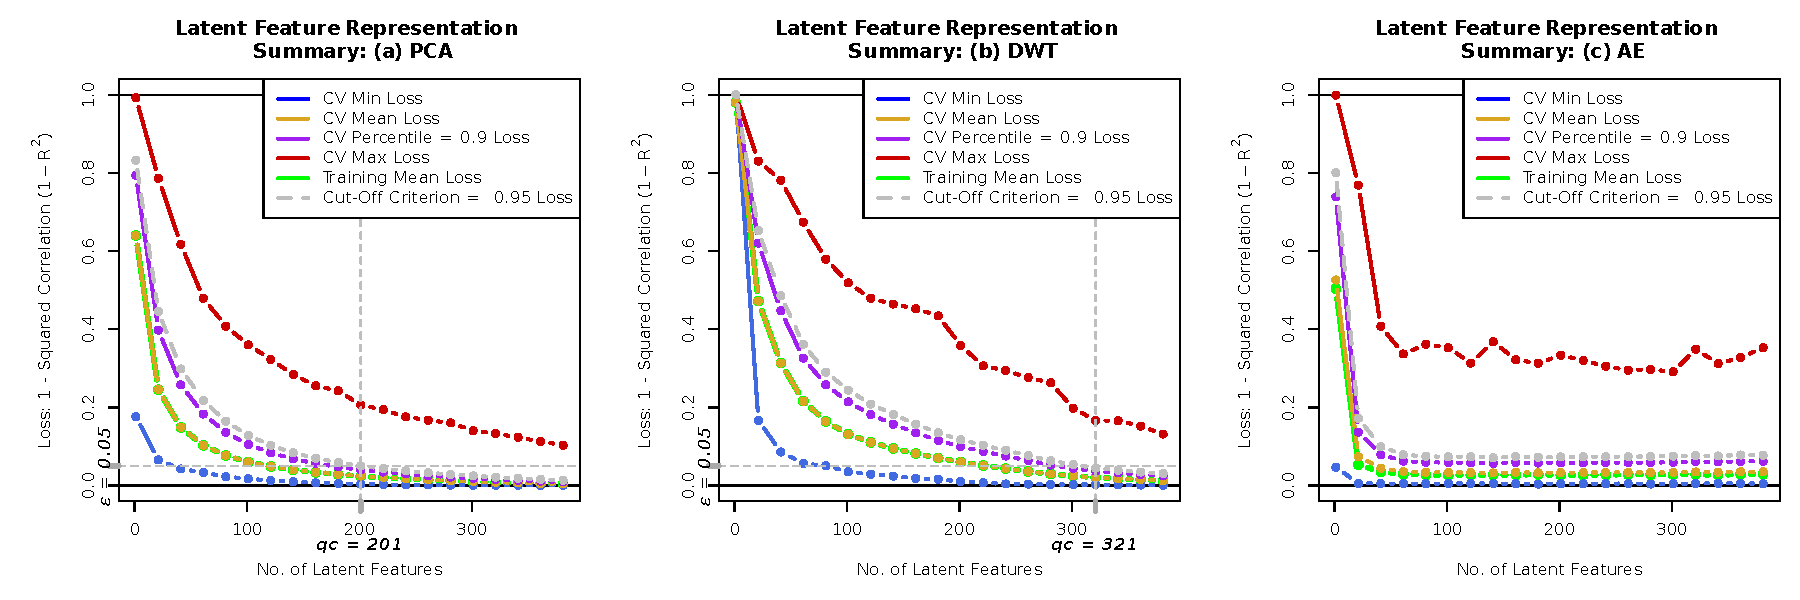
\includegraphics[width=1\textwidth]{figures/mnist-results.pdf}
    \caption{Summary \texttt{GLaRe()} plot for the MNIST data. A grid of equally-spaced values from $1$ to $381$ in increments of $20$ was used for the latent feature dimensions.}
    \label{fig:mnist-results}
\end{figure}


\subsection{Sample Size Experiment}\label{sec:sample-size-experiment}

We now present the results of an experiment that demonstrates the dependence of flexible latent feature representation methods such as PCA and AE on sample size.
In PCA, the encoding and decoding transformations are learned entirely from the data, so it is highly dependent on having a sufficient sample size.
In contrast, the DWT transformation is fixed a-priori and only the ordering of the wavelet coefficients to retain is learned from the data and hence there is less reliance on sample size.
We demonstrate this concept empirically on the Glaucoma dataset. 
We start with the full dataset ($N=306$) and then sub-sample the dataset to create smaller datasets of sizes $N=153$, $N=76$ and $N=38$ respectively.
We run \texttt{GLaRe()} to compare the performance of PCA and the thresholded DWT as the sample size is successively degraded.
In all cases, because of the small sample sizes, we use leave-one-out rather than $k$-fold cross-validation.

Figure \ref{fig:eye-sample-size-results-results-01} displays the results of the experiment.
The PCA results are displayed in the top row and the DWT results are displayed in the bottom row.
As PCA can only estimate, at most, $\min(N-1, T)$ features and in this case $N<T$, we see that the maximum possible number of latent features changes as the sample size decreases.
In contrast, there is no restriction on the number of latent features for the DWT and we manually choose a maximum of $K=500$, which is sufficient to achieve the qualifying criterion (with $\epsilon=0.05$ and $\alpha=0.95$) in all four cases.
The greater reliance of PCA on sample size is reflected in Figure \ref{fig:eye-sample-size-results-results-01} in several ways.
Firstly, the displayed quantiles of the cross-validated loss distribution, in particular the maximum, $0.95$ and $0.9$ quantiles (red, grey and purple lines) increase noticeably for PCA as the sample size is decreased, but they remain stable for the DWT.
The dependence is also reflected by the separation between the training and validation mean losses (green vs. yellow lines) as sample size is decreased, which demonstrates that PCA is unable to estimate a generalizable representation when the sample size is small, even if the training loss is satisfactory.
Finally, we can achieve the qualifying criterion using the DWT in all four cases (albeit with a large number of features), but we only achieve it for PCA with sample sizes $N=306$ and $N=153$.
The experiment is subject to sampling variability induced in the sub-sampling stage, so is repeated using a different random seed in Appendix \ref{sec:additional-results}.

\begin{figure}
    \centering
    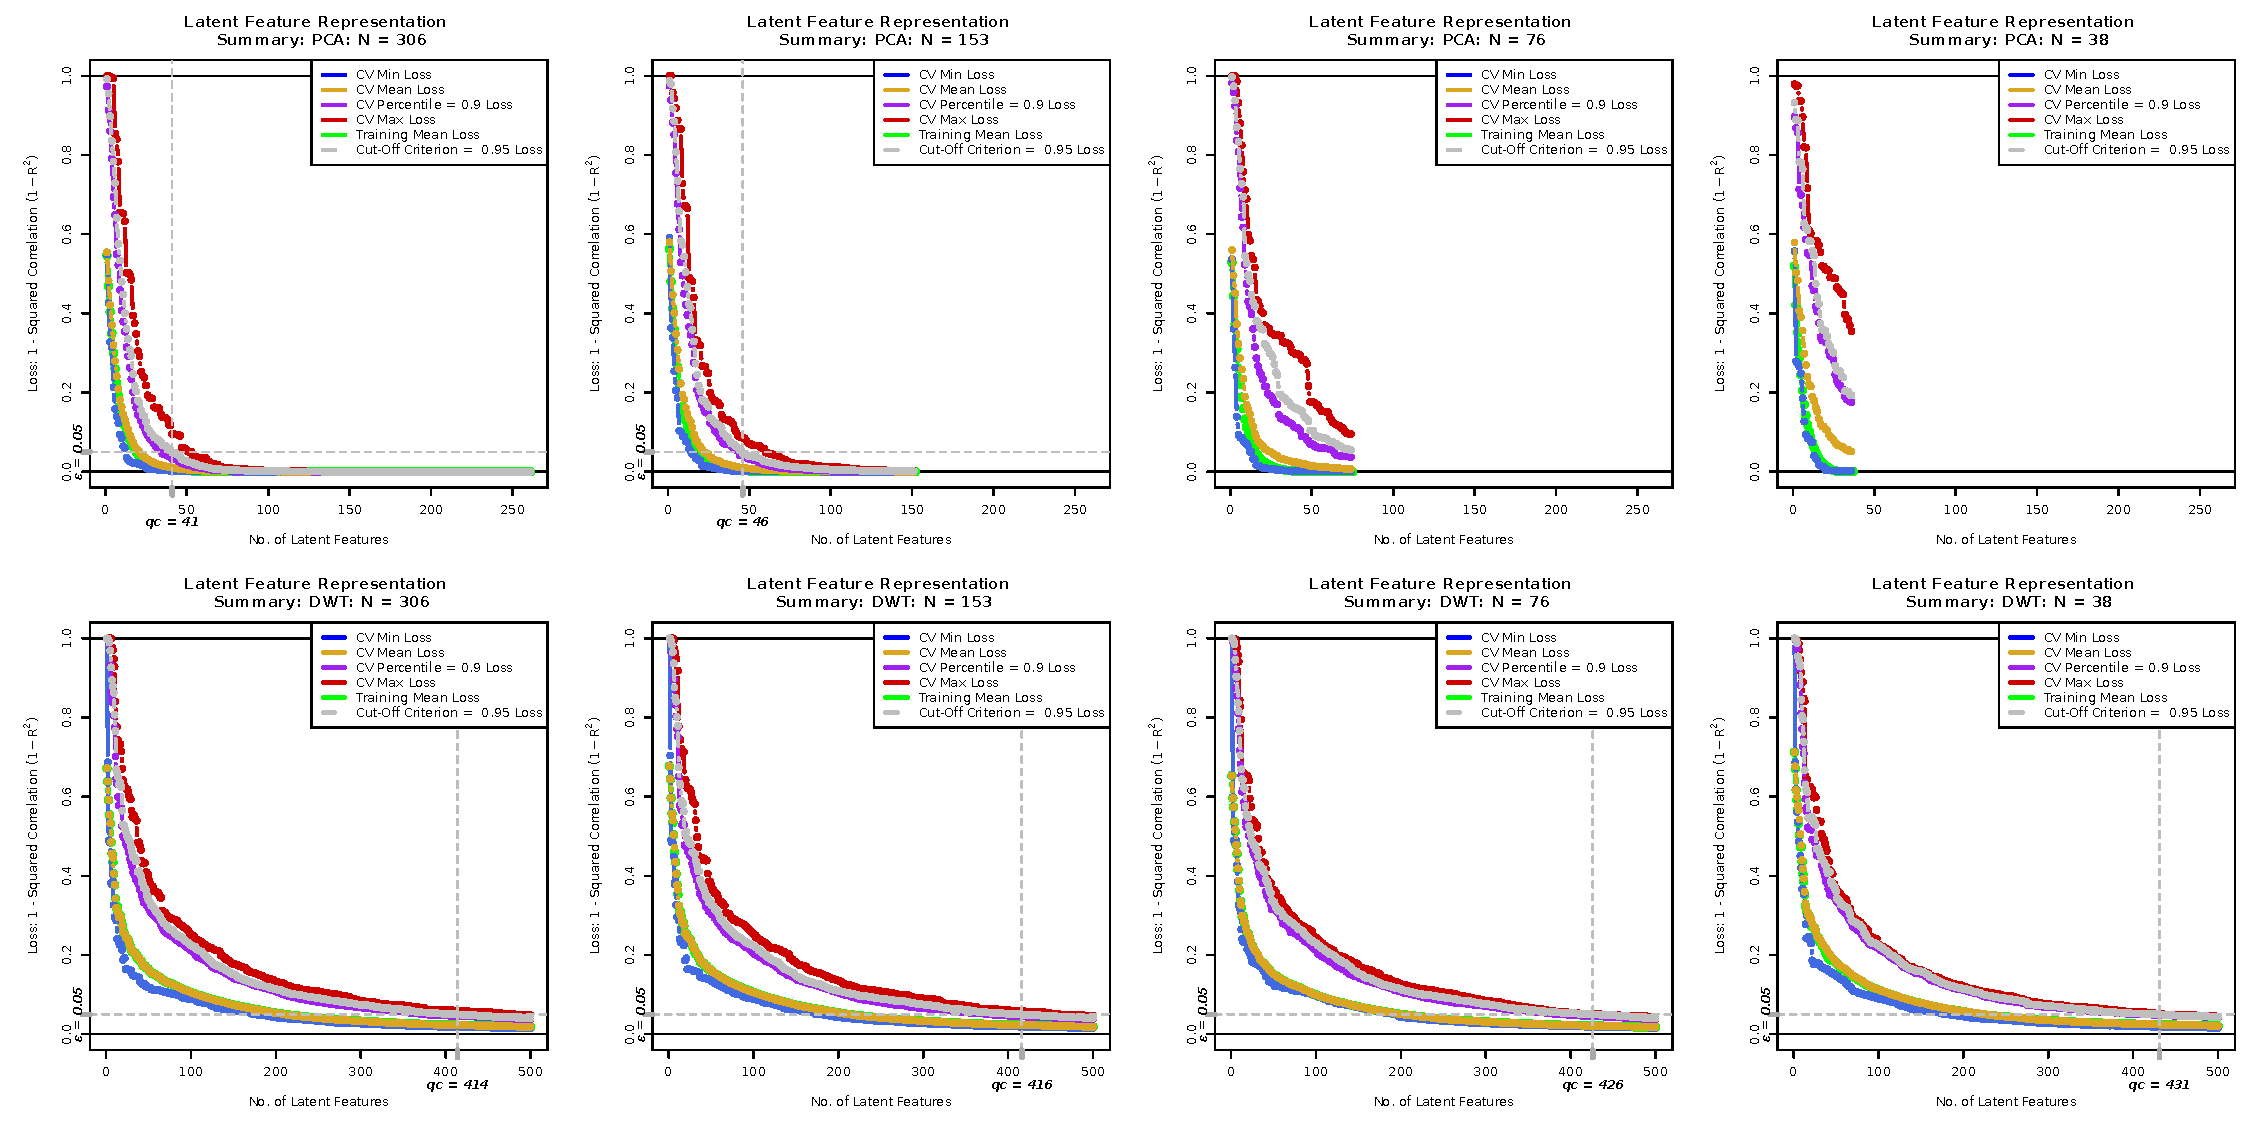
\includegraphics[width=1\linewidth]{figures/eye-sample-size-results-results-01.pdf}
    \caption{Results of the experiment to assess the effect of sample size on different latent feature representations. The Glaucoma data was used to create smaller datasets of size $N=153$, $N=76$ and $N=38$. \texttt{GLaRe()} was used to compare the representations provided by PCA (first row) and DWT (second row) as the sample size was decreased. Leave-one-out cross-validation was used in all cases.}
    \label{fig:eye-sample-size-results-results-01}
\end{figure}